\documentclass[times, utf8, zavrsni, numeric]{fer}
\usepackage{booktabs}
\usepackage{titlesec}
\newcommand{\sectionbreak}{\clearpage}
\frenchspacing
\begin{document}

% TODO: Navedite broj rada.
\thesisnumber{123456}

\title{Web aplikacija za predstavljanje portfelja programera}

\author{Mislav Vuletić}

\maketitle

\zahvala{}
Posvećeno svima koji su voljni učiti i neprestano napredovati.

\tableofcontents

\chapter{Uvod}
\qquad Prilikom traženja posla prednost je ako se programer može predstaviti potencijalnom poslodavcu sa svim projektima u kojima je sudjelovao i programskom podrškom koju je razvio.
Često se za tu svrhu koriste LinkedIn\footnotemark{} ili Git\footnotemark{} stranice, odnosno druge vlastite web stranice programera.
\footnotetext{LinkedIn - poslovno orijentirana socijalna mreža}
\footnotetext{git - sustav za upravljanje izvornim kodom nastao 2005.~godine}
Učinkovito predstavljanje može se postići uz pomoć jedne web stranice koja će omogućavati pregled projekata kroz Git alate, sadržavati linkove na aktivne projekte te omogućiti međusoban kontakt programera i poslodavca putem korisničkog sučelja.

Ovaj rad prolazi kroz postupak postavljanja aktivne web stranice programera.
Fokus rada nije na izradi najjednostavnije realizacije cilja nego izrada skalabilnog rješenja kojim se funkcionalnost stranice može proširiti u bilokojem trenutku.

\chapter{Ideja}
\section{Funkcionalni i nefunkcionalni zahtjevi}
\subsection{Funkcionalni zahtjevi}
\qquad Vlastita portfolio web stranica programera mora sadržavati opis programera, njegove kontaktne informacije te brze poveznice na stranice git repozitorija i stranice socijalnih mreža.
Programsko rješenje mora posjedovati mogučnost komunikacije s programerom direktno na stranici, poput slanja mail poruke.
Nadalje, web stranica mora imati sistematičan odjeljak za projekte na kojima je programer radio.
To znači da svaki projekt mora imati svoje mjesto na stranici koje će sadržavati ime projekta, kratki opis projekta, sliku projekta te mogući daljnji sadržaj prema potrebi.
Na stranici mora postojati način posluživanja CV dokumenta, odnosno životopisa u pdf formatu.

\subsection{Nefunkcionalni zahtjevi}
\qquad Vlastita portfolio web stranica programera mora koristiti vlastitu domenu programera.
Mora biti podignuta na udaljenom poslužitelju, odnosno serveru.
Stranica mora biti moderna i jednostavna.
To znači da mora biti privlačna potencijalnom poslodavcu.
Web sjedište također mora biti jednostavno i intuitivno za korištenje, što podrazumijeva brze poveznice za laku navigaciju.

\section{Istraživanje i sakupljanje informacija}
\subsection{Portfolio stranice nekih programera}
\qquad Prije kretanja na posao smišljanja vlastitog uređenja stranice cilj je bio istražiti kako su drugi programeri postigli učinak privlačenja pažnje potencijalnih poslodavaca.
Stranica \textit{www.creative-portfolios.com} nam je uvelike olakšala posao obzirom da se održava dnevno te se mogu pratiti promjene na stranicama github-a.
Web sjedišta koja se posebno ističu su: \textit{cihadturhan.com}, \textit{fishnation.de} te \textit{eli.wtf}.
Ono što ove stranice čini vrijedne izbora je autentičnost te vrlo intuitivno pronalaženje informacija. Slika 2.1 prikazuje zaslon trenutnih vještina programera sa stranice \textit{cihadturhan.com}.

\begin{figure}[htb]
				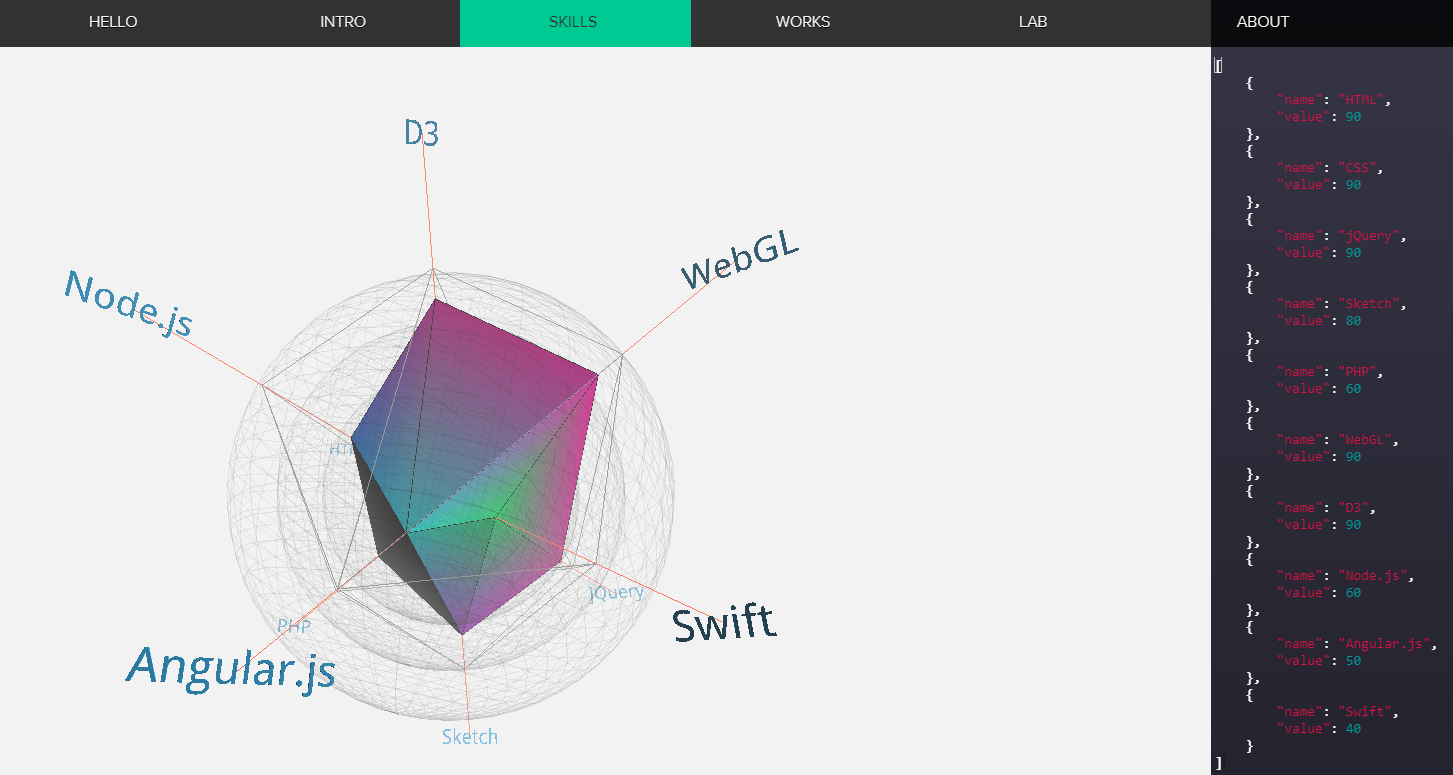
\includegraphics[width=14.6cm]{images/skills.png}
				\caption{Slika 2.1 vještine programera}
				\label{fig:skills}
\end{figure}

\chapter{Tehnologije rješenja}
\section{Jezik i generiranje pogleda}
\subsection{Programski jezik Java}
\qquad Java je objektno orijentirani programski jezik razvijen iz programskoj jezika Oak\footnotemark{}.
\footnotetext{Oak - programski jezik razvijen 1991., evoluirao u programski jezik Java 1995.}
Centralna ideja u razvoju programskog jezika Java bila je potpora za više platformnost.
Tako se danas Javin virtualni stroj može vrtiti na gotovo svim platformama; od Linuxa, Solarisa, Mac OS-a do Windowsa.
Druga bitna stavka je da je Java programerima potpuno nebitno hoće li se njihov program izvoditi na 32-bitnom ili 64-bitnom sustavu.
To je zato što Javina specifikacija definira apstraktni računski virtualni stroj kod kojeg je sve propisano.
\subsection{Thymeleaf}
\qquad Thymeleaf je moderan skup modela za razvitak samostojećih web aplikacija koji se vrti na poslužitelju.
Služi za serviranje XHTML ili HTML5 datoteka.
Thymeleaf teži potpuno nadomjestiti \textit{JSP}\footnotemark{}, te učiniti tehnologiju jednostavnijom za korištenje.
\footnotetext{JSP - Java Server Pages, služi dinamičkom generiranju HTML, XML i drugih tipova datoteka}
Glavni razlog korištenja Thymeleaf-a jest što nudi elegantna rješenja za razvojni tijek rada kroz HTML.

\section{Java Spring Model-View-Controller}
\qquad Java Spring MVC je modul vrlo popularnog \textit{framework}-a\footnotemark{} Java Spring koji je zaživio u prvom desetljeću 21.~stoljeća.
\footnotetext{framework - radni okvir, definira strukturu, odnosno temelje aplikacije}
Java Spring je \textit{open-source}\footnotemark{} biblioteka za Java platformu.
\footnotetext{open-source - dostupan javnosti na uvid, korištenje, izmjene i daljnju distribuciju}
Omogučava lakši razvoj standardnih i \textit{enterprise}\footnotemark{} aplikacija.
\footnotetext{enterprise aplikacije - prevelika i prekompleksna aplikacija za individualno korištenje}
Java Spring MVC koristi popularnu strategiju izrada web stranica.
MVC definira tri cjeline; \textit{\textbf{M}odel} (model), \textit{\textbf{V}iew} (pogled), \textit{\textbf{C}ontroller} (upravitelj).
\begin{figure}[htb]
				\centering
				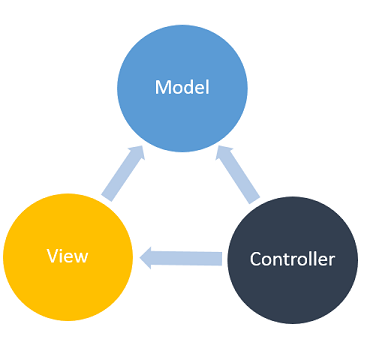
\includegraphics[width=5cm]{images/mvc.png}
				\caption{MVC struktura}
				\label{fig:mvc}
\end{figure}

\noindent
Ideja svake od tih cjelina je jasno odrediti gdje se koji dio aplikacije treba nalaziti.
\begin{itemize}
				\item Model uključuje \textit{backend}\footnotemark{}, te podatke aplikacije, odnosno poslovnu logiku i bazu podataka ako je aplikacija ima.
		\footnotetext{backend - pomoćni sustav, server}
	\item View (pogled) je dio koji korisnik naše aplikacije vidi; 
		html\footnote{html - Hyper Text Markup Language, prezentacijski jezik za izradu web stranica}, 
		css\footnote{css - Cascading Style Sheets, stilski jezik koji služi opisu html dokumenta}, 
		javascript\footnote{javascript - skriptni programski jezik koji se izvršava u web pregledniku}.
	\item Controller (upravitelj) upravlja korisničkim zahtjevima.
\end{itemize}
Dodatno Java Spring definira HandlerAdapter, HandlerInterceptor, HandlerMapping, LocaleResolver, MultipartResolver te ViewResolver koji definiraju gdje se dijelovi koda moraju nalaziti za lakše održavanje i razvitak EE\footnotemark{} aplikacija.
\footnotetext{EE - \textit{enterprise edition}, odnosno aplikacije velikog spektra}

\section{Pokretanje aplikacije na poslužitelju}
\subsection{Digital Ocean}
\qquad Digital Ocean je servis koji nudi najam poslužiteljskih računala na njihovom oblaku.
Sjedište im je u New York-u, no imaju servere u cijelom svijetu što dopušta korisnicima da postave svoju aplikaciju na više lokacija po svijetu kako bi se njihova web stranica brže učitavala.
\subsection{Apache Tomcat}
\qquad Apache Tomcat program je \textit{open source} implementacija Javinih servleta te \textit{JSP}\footnotemark{}, \textit{JEL}\footnotemark{} i \textit{JWS}\footnotemark{} specifikacija razvijenih od Java programera.
\footnotetext{JSP - Java Server Pages}
\footnotetext{JEL - Java Expression Language}
\footnotetext{JWS - Java WebSocket}
Služi kao potpuno Java okruženje za izvođenje HTTP web okruženja na kojima se Java kod može izvoditi.

\section{Korištene biblioteke}
\subsection{SimpleGrid.css}
\qquad Simple Grid je jednostavna css mreža koja nudi podjeljivanje stranice u 12 stupaca.
Napravljena je s pogledom na mobitelu na prvom mjestu te se svi stupci protežu do rubova ekrana na manjim ekranima.
U našem projektu ova biblioteka se koristi na stranici \textit{/projects} za jednostavniji razmještaj elemenata u web pregledniku.
\subsection{fullPage.js}
\qquad FullPage.js je tehnologija koja omogučava korisniku da vrlo jednostavno postavi web stranicu na kojoj je omogučeno pomicanje za cijelu stranicu koristeći \textit{scroll} tipku\footnotemark{} na mišu.
Tehnologija je vrlo popularna te je koriste kompanije poput Google, Coca Cola, Ebay, itd.
\footnotetext{scroll - gumb klizaća, nalazi se između lijeve i desne tipke na mišu}
\subsection{Google fonts}
\qquad Google fonts je kolekcija interaktivnih sučelja koje omogučuju korisniku odabir fonta za tekst koji se nalazi na njegovoj stranici.
Usluga je podržana od kompanije Google te se ne naplaćuje niti sama usluga niti brzina dohvaćanja fonta s njihovih poslužiteljskih računala.
\subsection{CodePen api}
\qquad CodePen je socijalno mrežno okruženje za razvijanje jednostavnih programa koristeći \textit{html}, \textit{css} i \textit{javascript} direktno u web pregledniku.
Okruženje se sastoji od četiri polja, gdje tri od ta četiri pripadaju jezicima navedenima prije, a zadnje polje služi pregledu rezultata.
CodePen sučelje dozvoljava ugradnju tog okruženja u vlastitu stranicu.
\subsection{SvgBackgrounds}
\qquad SvgBackgrounds je priključak za web aplikacije.
Omogučava postavljanje \textit{SVG}\footnotemark{} pozadina veličine 5KB te je podržan od većine web preglednika koji se danas koriste.
\footnotetext{SVG - slike određene vektorima u XML formatu}

\chapter{Opis rješenja}
\section{Početna stranica}
\qquad Početna stranica nalazi se na poveznici \textit{mmedo.me}.
\section{Stranica za slanje poruke}
\qquad Stranica za slanje poruke sadrži poveznicu za povratak na početnu stranicu te prostor za unos poruke i tipku za slanje poruke. Slika prikazuje stranicu sa primjerom poruke koji se nalazi na stranici pri učitavanju.

\begin{figure}[htb]
				\centering
				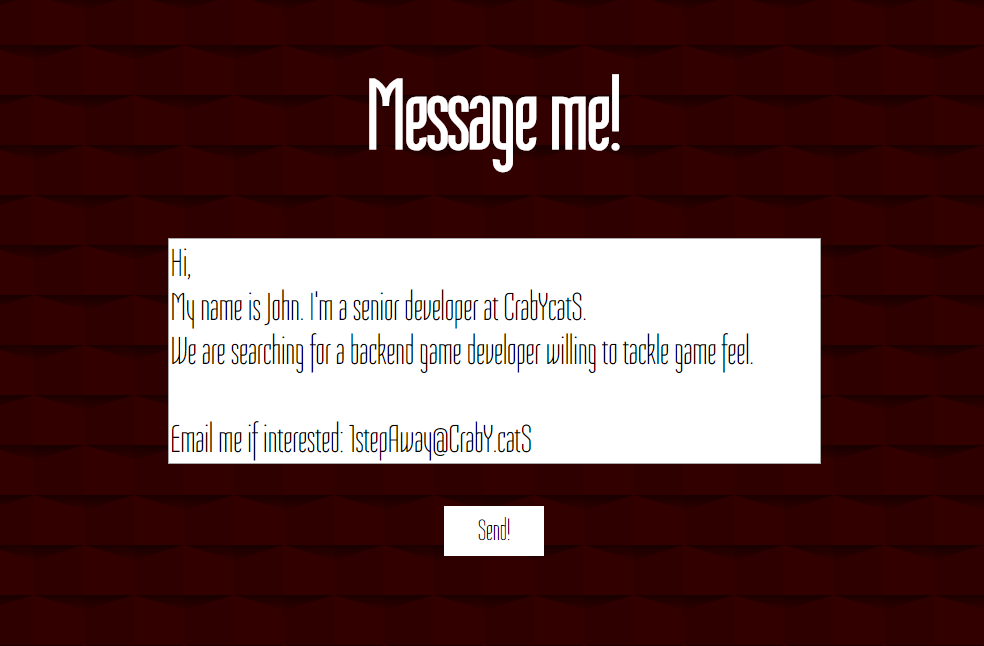
\includegraphics[width=14.6cm]{images/message.png}
				\caption{Slika stranice za slanje poruke}
				\label{fig:message}
\end{figure}

\section{Stranica opisa programera}
\qquad Stranica opisa programera nalazi se na poveznici \textit{mmedo.me/about}.

\section{Dohvat životopisa programera}
\qquad Pri paljenju aplikacija iz memorije se s diska učitava pdf datoteka u bajtovima.
No kako doći do nje korištenjem stranice?
Na početnoj stranici se pritisne na brzu poveznicu \textit{resume}.
Tada aplikacija prosljeđuje zahtjev drugom kontroleru na poveznicu \textit{mmedo.me/resume} 
Kontroler učitano polje bajtova pohranjuje u http zaglavnje u kojem postavlja tip datoteke na pdf, te upute da datoteku web preglednik ne treba skinuti nego direktno prikazati u web pregledniku s ugrađenim pdf preglednikom.
Ukoliko korišteni web preglednik nema ugrađen pdf preglednik datoteka će biti skinuta na disk.

\section{Stranica projekata}
\qquad Stranica projekata nalazi se na poveznici \textit{mmedo.me/projects}.
Stranicu projekata možemo zamisliti kao dvodimenzionalni koordinatni sustav.
Pomicanjem po ordinati koordinatnog sustava listamo projekte.
Pomicanjem po apscisi koordinatne mreže listamo pojedinosti odabranog projekta.
Takav pristup omogučen je korištenjem \textit{fullpage.js} biblioteke.
Ona nam omogučava sigurnost da klizačem ne možemo dospjeti između dva polja u našoj koordinatnoj mreži.

\section{Stranica pogreške}
\qquad Stranica pogreške nalazi se na \textit{mmedo.me/error} no svi nepostojeći linkovi također vode na tu stranicu.

\chapter{Zaključak}

\bibliography{literatura}
\bibliographystyle{fer}
\begin{thebibliography}{9}
\bibitem{programiranje-u-javi}
				Marko Čupić.
				\textit{Programiranje u Javi}.
				Inačica 30. rujna 2015.

\bibitem{awesome-portfolios}
				Awesome Creative Portfolio Websites,
				\\\texttt{github.com/iRaul/awesome-portfolios},
				\\\texttt{www.creative-portfolios.com}

\bibitem{java-spring}
				Spring by Pivotal,
				\\\texttt{spring.io}

\bibitem{w3schools}
				W3Schools Online Web Tutorials
				\\\texttt{https://www.w3schools.com/}

\bibitem{stackoverflow}
				StackOverflow,
				\\\texttt{https://stackoverflow.com/}

\bibitem{svgbackgrounds}
				SVGBackgrounds,
				\\\texttt{https://www.svgbackgrounds.com/}

\bibitem{three-image-transition}
				THREE Image Transition,
				Szenia Zadvornykh.
				\texttt{https://codepen.io/zadvorsky/pen/PNXbGo}

\bibitem{}
\bibitem{}
\bibitem{}
\bibitem{}
\bibitem{}
\bibitem{}
\end{thebibliography}

\begin{sazetak}
\qquad Rad predstavlja izradu vlastite web stranice.

\kljucnerijeci{Java, Java Spring, Spring, MVC, portfolio, web, web stranica, portfelj, vlastita web stranica, web stranica programera, javascript}
\end{sazetak}

\engtitle{Software Developer Portfolio Web Application}
\begin{abstract}
Abstract.

\keywords{Java, Java Spring, Spring, MVC, portfolio, web, website, site, developer website, javascript}
\end{abstract}

\end{document}
